\section{Software Stack}
For software development on the proposed system we have developed an initial software infrastructure to support the development of complex applications.
This software stack builds on the existing RISC-V software infrastructure with modifications to support the proposed accelerator.
Specifically, we modify LLVM 15.0 to emit the RoCC instructions mentioned in the previous section and develop a low-level user library to invoke those functions.
On top of this low-level library we build custom BLAS-like kernels for matrix-vector and matrix-matrix operations, and use OpenMP to distribute tasks across the tiles of the proposed system.  

\begin{figure}[ht]
\centering
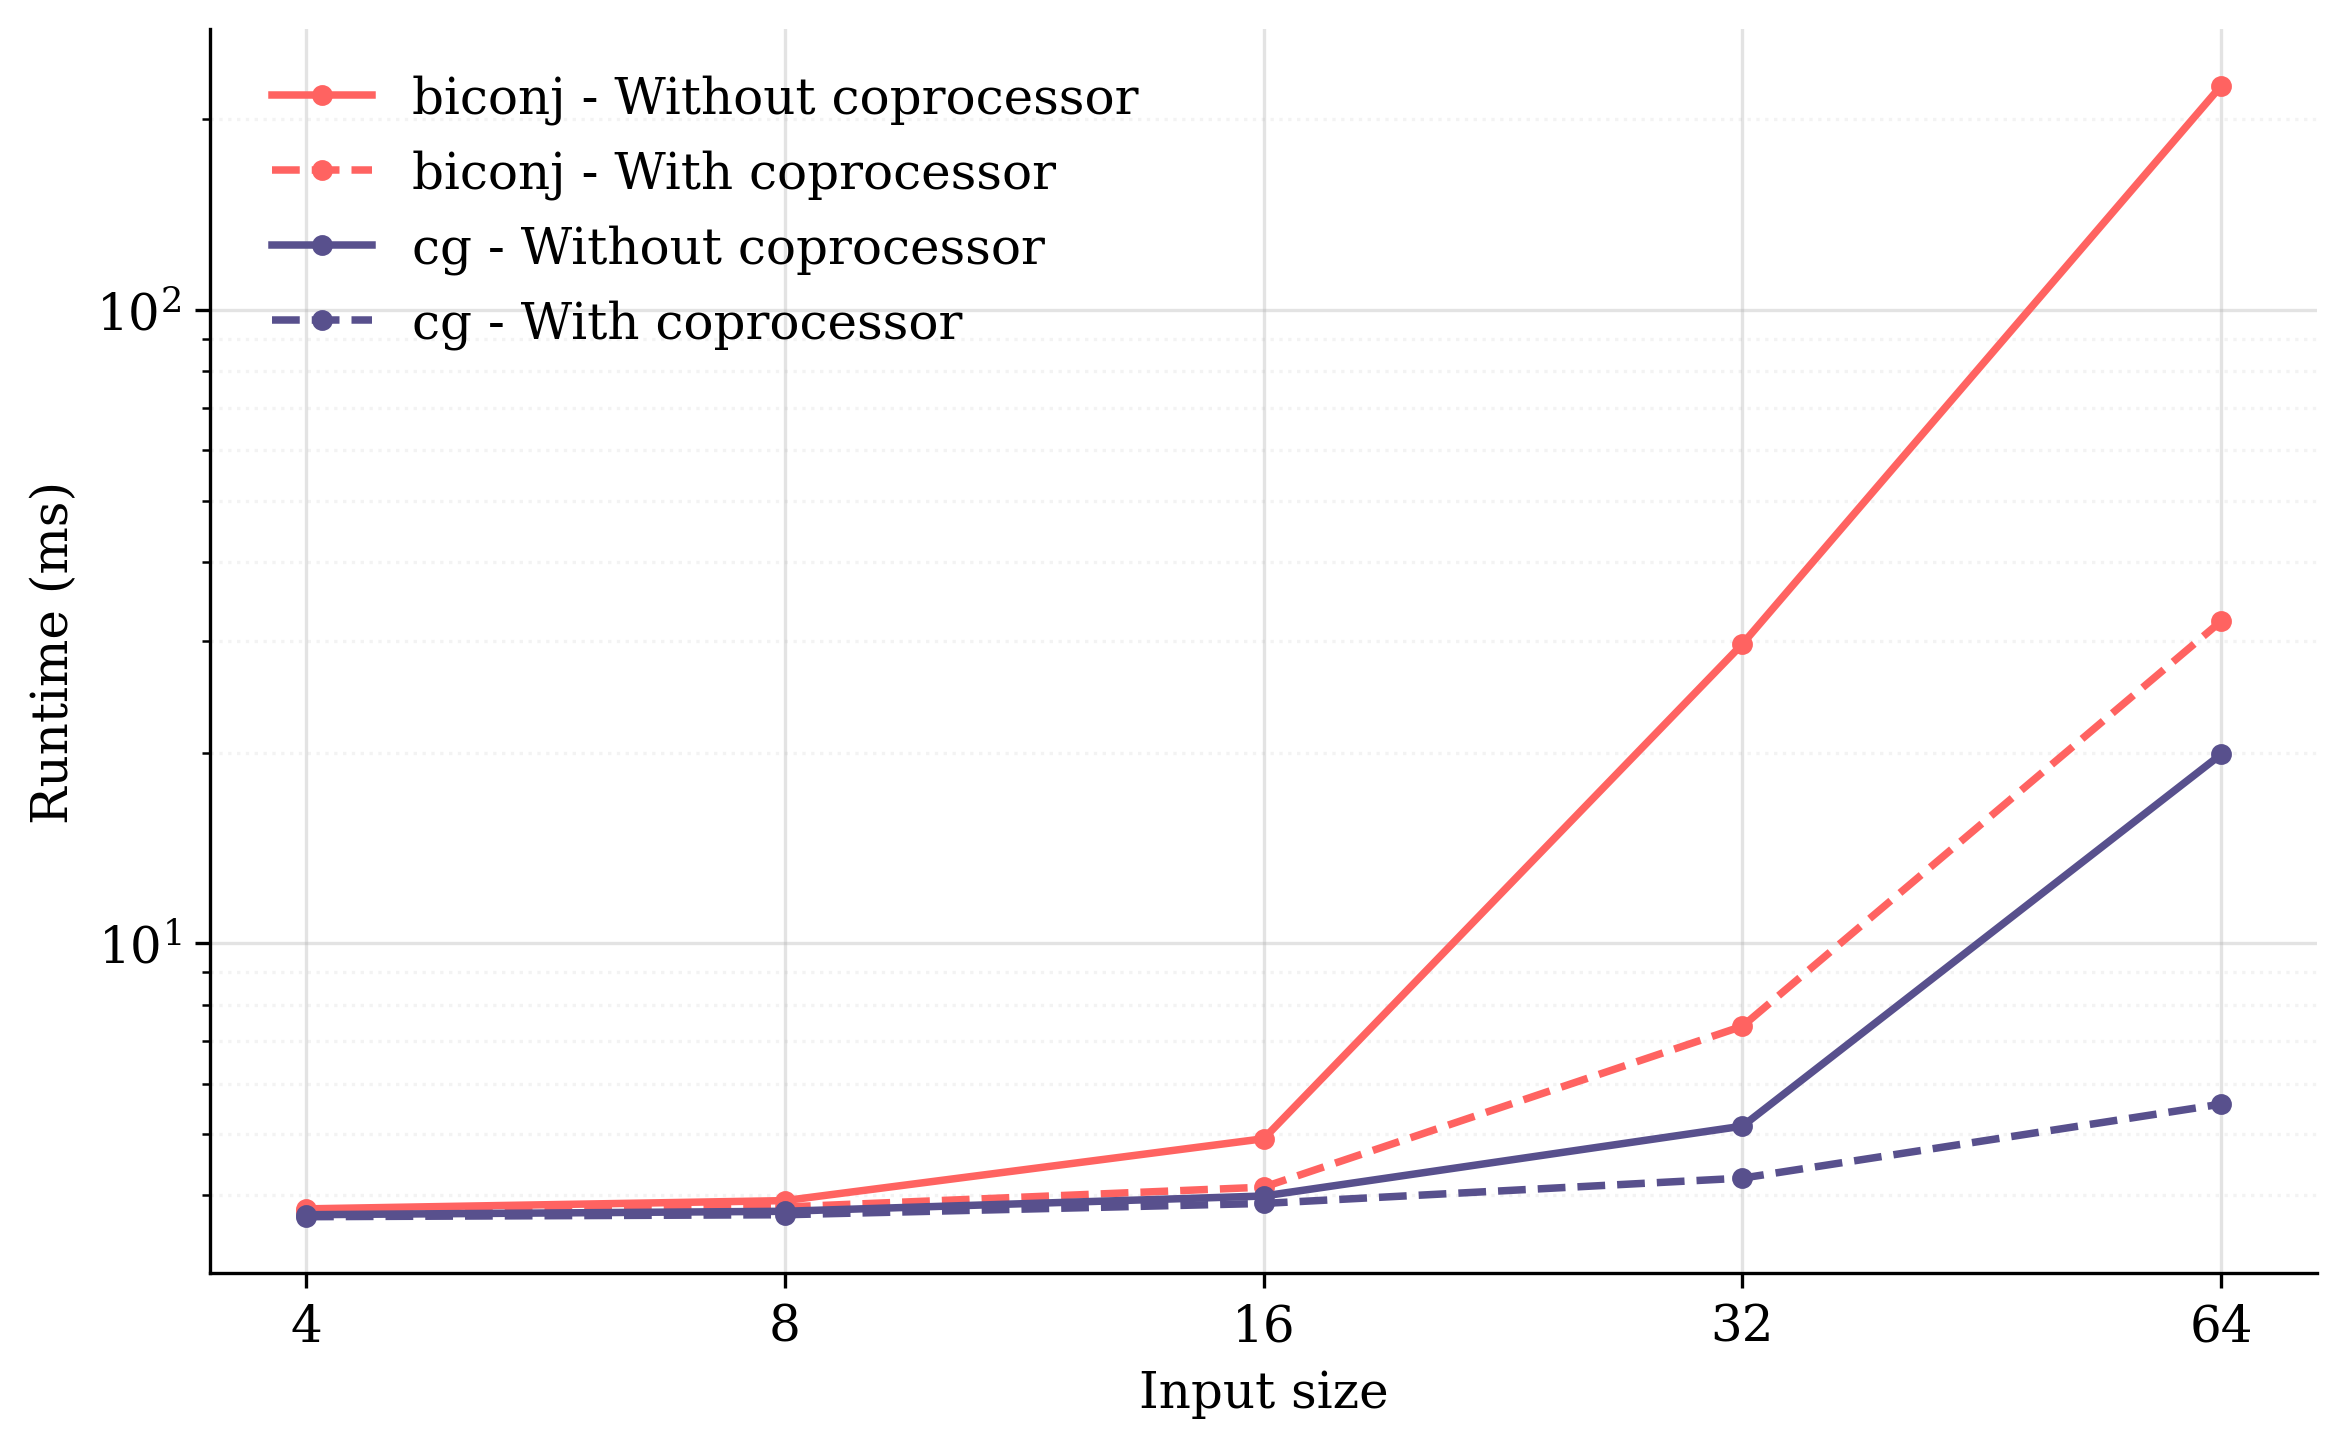
\includegraphics[scale=0.42]{figures/with_without.png}
\vspace{-10pt}
\caption{Runtime Comparison of CG + BiCGStab as N grows}
\vspace{-10pt}
\label{fig:single}
\end{figure}

\subsection{Analog BLAS}
Given the ubiquity of BLAS in HPC applications, we select it as the primary user-facing interface to the analog arrays.
Importantly, we only implement BLAS kernels that can be readily mapped to the proposed analog coprocessor, specifically \texttt{gemm} and \texttt{gemv} in both real and complex variations.
%TODO: Cite to complex expansion if space
In addition to providing a well-known interface, these functions also perform two essential operations for the analog coprocessor, scaling, and size-agnostic mapping.

Analog arrays typically require some form of scaling for optimal performance.
When using a fixed-point interface, values must be scaled into the range of [-1,1] or [0,1] to ensure that the underlying analog ranges are fully used.
With a floating-point interface as evaluated here, scaling is less essential; however, it can take load off of the hardware floating-pointing emulation within the coprocessor.

Unlike digital systems where BLAS functions can take arbitrarily sized matrices, each tile's analog coprocessor has a maximum supported matrix size.
Moreover, matrices and vectors which are not integer multiples of the underlying array size require partitioning and/or zero-padding for mapping to a given array.

To handle both of these operations, the developed AnalogBLAS functions used a specialized \texttt{AnalogMatrix} object to provide an interface for programmed arrays.
Internally AnalogMatrices allocate arrays from a tile coprocessor's pool, track which array identifiers are associated with each matrix, and track scale factors which are used to undo scaling operations providing the programmer with a transparent interface to the BLAS functions.
Importantly, in our current implementation a given tile can only allocate arrays within the tile, support for problems spanning multiple tiles is handled through OpenMP.

\subsection{Multi-tile Operations using OpenMP}

To scale problems beyond a single tile, we use an unmodified RISC-V OpenMP implementation.
Importantly, in the current implementation matrices and inputs are manually partitioned such that each tile's portion of the matrix is at most the maximum matrix capacity of each tile based on the number of analog arrays.
This leads to an interesting insight for analog acceleration for HPC workloads, the use of analog arrays implies that the system must use weak rather than strong scaling.
Although it is possible to reduce the overall portion of the problem allocated to each tile, under-utilizing arrays creates significant inefficiencies which should be avoided.

\begin{figure}[ht]
    \centering
    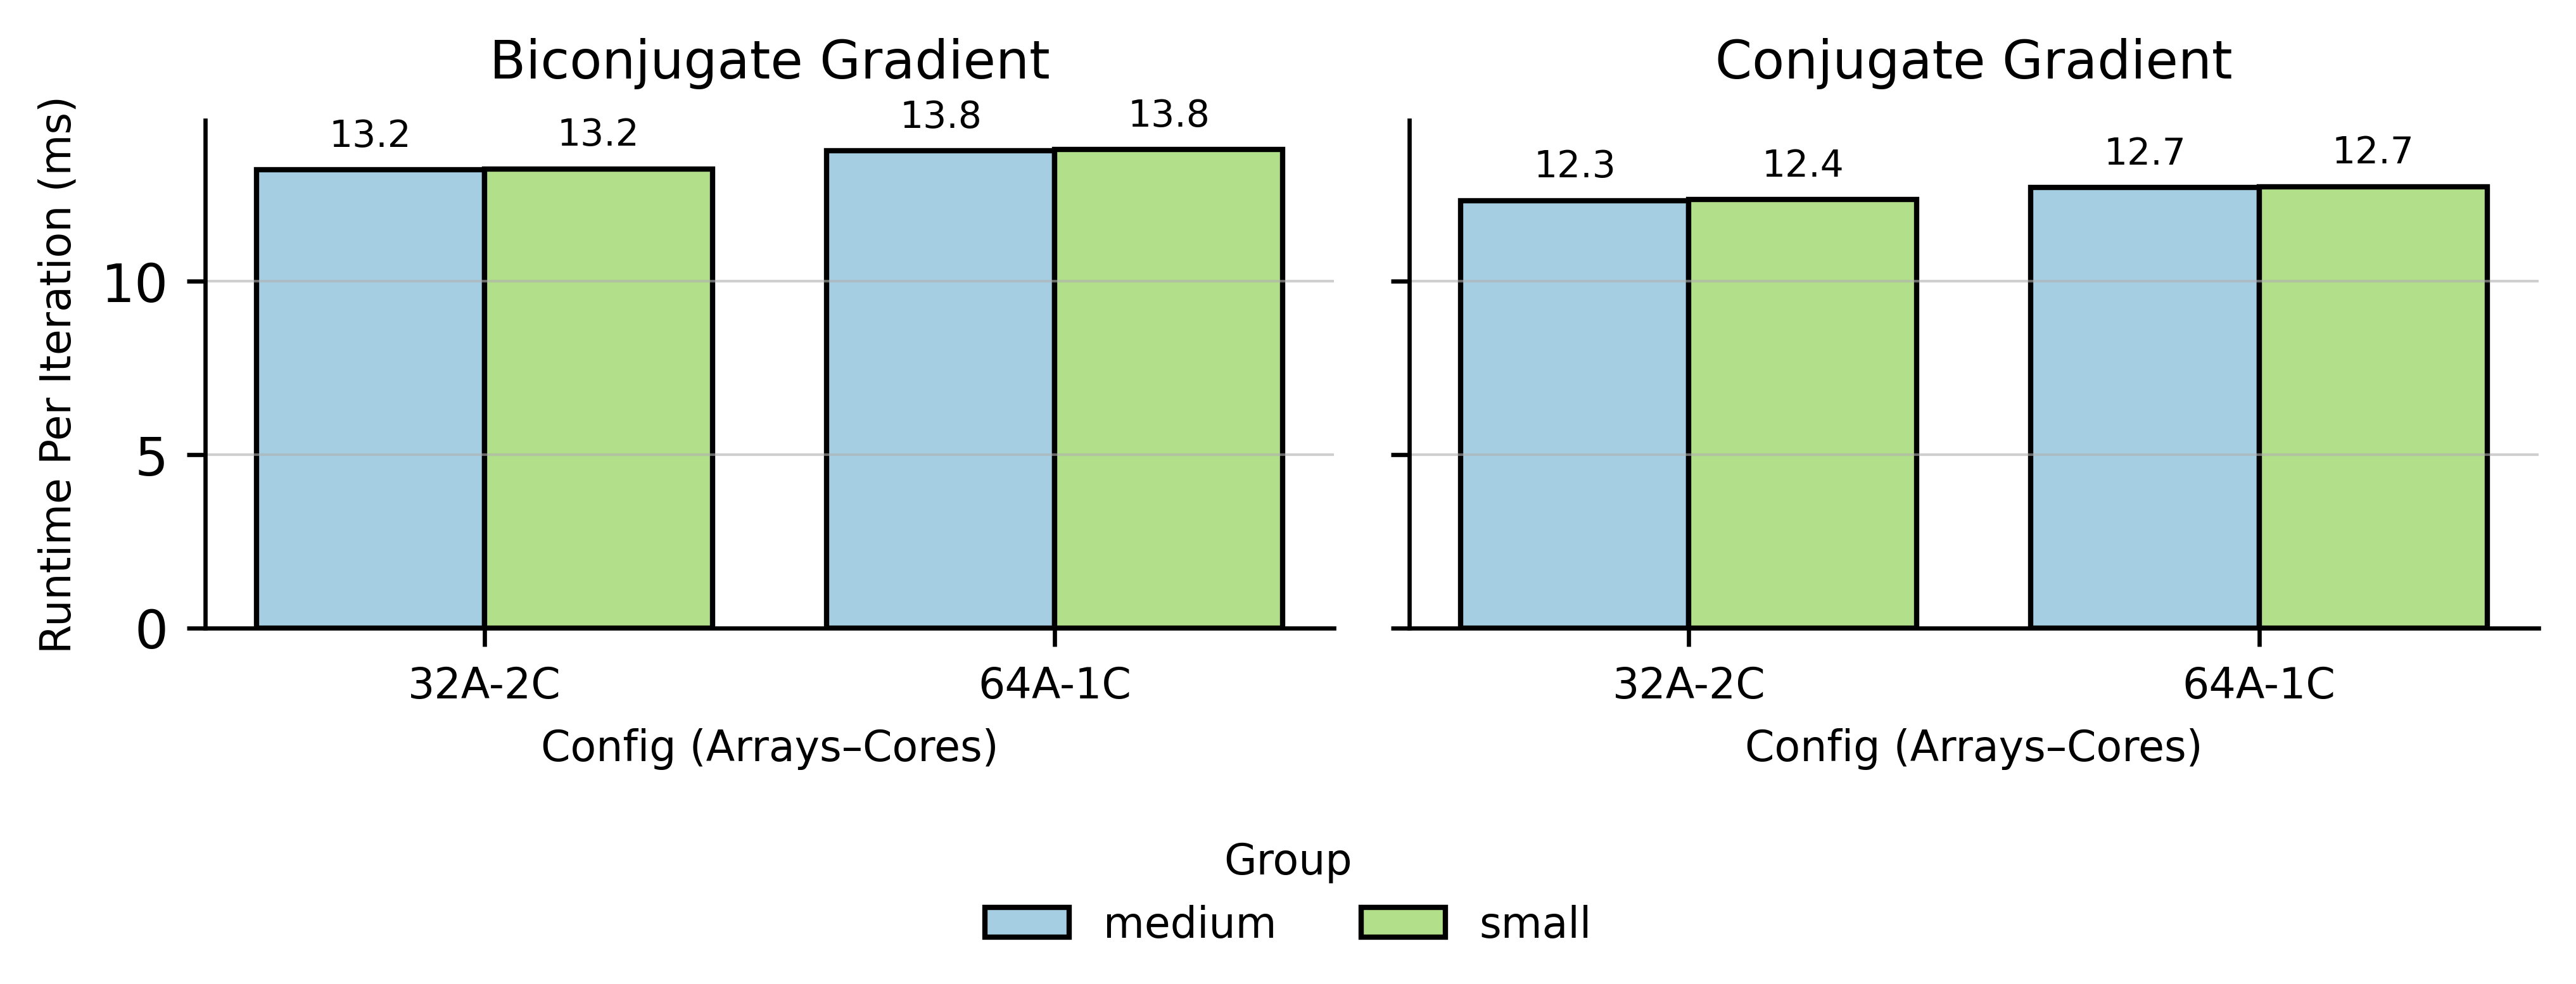
\includegraphics[scale=0.42]{figures/results.png}
    \vspace{-10pt}
    \caption{Runtime Comparison of CG + BiCGStab}
    \label{fig:array_core}
    \vspace{-18pt}
\end{figure}

\subsection{Implementing Iterative Linear Solvers}

Using our Analog BLAS implementation and OpenMP the iterative solvers we implement a pair of iterative linear solvers, Conjugate Gradient CG and BiCG-Stab.
The matrix is partitioned with a two level recursive partitioning, first allocating contiguous blocks to the tiles, and subsequently partitioning those blocks across multiple arrays.
CG and BiCG are the same solvers implemented by Feinberg et al., in prior work~\cite{8416841}; however, by building on the RISC-V software stack we are able to build a more robust and extensible implementation using standard libraries. 